\documentclass{sig-alternate}
\usepackage[utf8]{inputenc}
\usepackage[T1]{fontenc}

\newcommand{\superscript}[1]{\ensuremath{^{\textrm{#1}}}}
\def\sharedaffiliation{\end{tabular}\newline\begin{tabular}{c}}
\def\wu{\superscript{*}}
\def\wg{\superscript{\dag}}

\usepackage{listings} 

% Typography
\usepackage{times}
\usepackage{mathptmx}
\usepackage{microtype}
\usepackage[normalem]{ulem}
\usepackage[pdftex,bookmarks,bookmarksopen,bookmarksdepth=2,
            urlcolor=black,colorlinks=true,linkcolor=black,citecolor=black]{hyperref}
\usepackage[capitalize,noabbrev]{cleveref}
\def\UrlFont{\em}

% Graphics
\usepackage{tikz}
\usepackage{tkz-graph}
\usetikzlibrary{arrows,positioning,shapes.misc}
\usepackage{graphicx}
\definecolor{lightgrey}{RGB}{170, 170, 170}
\definecolor{darkblue}{RGB}{0, 0, 0}
\definecolor{darkred}{RGB}{170, 0, 0}
\definecolor{darkgreen}{RGB}{0, 110, 0}

% Acronyms
\usepackage{xspace}
\newcommand{\sparql}{{SPARQL}\xspace}
\newcommand{\sparqlo}{{SPARQL 1.1}\xspace}
\newcommand{\arq}{{ARQ}\xspace}
\newcommand{\wthreec}{{W\oldstylenums 3C}\xspace}
\newcommand{\sfive}{{S\oldstylenums 5}\xspace}
\newcommand{\select}{{SELECT}\xspace}
\newcommand{\construct}{{CONSTRUCT}\xspace}
\newcommand{\ask}{{ASK}\xspace}
\newcommand{\describe}{{DESCRIBE}\xspace}
\newcommand{\from}{{FROM}\xspace}
\newcommand{\odbc}{{odbc}\xspace}

% Tight lists
\usepackage{enumitem}
\setlist{nolistsep}

% Listings and Verbatim environment
\usepackage{fancyvrb}
\usepackage{relsize}
\usepackage{listings}
\usepackage{verbatim}
\newcommand{\smalllistingsize}{\fontsize{8pt}{9.5pt}}
\newcommand{\inlinelistingsize}{\fontsize{8.5pt}{11pt}}
\newcommand{\defaultlistingsize}{\inlinelistingsize}
\RecustomVerbatimCommand{\Verb}{Verb}{fontsize=\inlinelistingsize}
\RecustomVerbatimEnvironment{Verbatim}{Verbatim}{fontsize=\inlinelistingsize}
\lstset{frame=lines,captionpos=b,numberbychapter=false,escapechar=§,
        belowskip=1em,
        xleftmargin=2ex,
        framexleftmargin=2ex,
        basicstyle=\ttfamily\smalllistingsize\selectfont}
\crefname{lstlisting}{Listing}{Listings}
\definecolor{grey}{RGB}{130,130,130}

\usepackage{color}
\newcommand{\todo}[1]{\noindent\textcolor{red}{{\bf \{TODO}: #1{\bf \}}}}
\begin{document}

\title{What we can learn from one year of\\ public transit route planning API queries}
\numberofauthors{6}
\author{
\alignauthor
Pieter Colpaert\\
\affaddr{\email{\texttt{pieter.colpaert@ugent.be}}}
\and
\alignauthor
Alvin Chua\\
\affaddr{\email{\texttt{alvin.chua@asro.kuleuven.be}}}
\and
\alignauthor
Ruben Verborgh\\
\affaddr{\email{\texttt{ruben.verborg@ugent.be}}}
\and
\alignauthor
Erik Mannens\\
\affaddr{\email{\texttt{erik.mannens@ugent.be}}}
\and
\alignauthor
Rik Van de Walle\\
\affaddr{\email{\texttt{rik.vandewalle@ugent.be}}}
\and
\alignauthor
Andrew Vande Moere\\
\affaddr{\email{\texttt{andrew.vandemoere\\@asro.kuleuven.be}}}\\
}

\maketitle
\begin{abstract}
% Context
%Public transit schedules are made available on the Web in various ways, such as in a GTFS file, a route planning API, or through Linked Connections.
The iRail project hosts a route planning API for the Belgian railway company.
This webservice provides a concise answer to a complex question with parameters such as ``departuretime'', ``from'' and ``to''.
% Need
In the field of urban planning, researchers need an indication of how people move between cities. 
Yet, getting this data from official sources has proven to be troublesome.
% Task
In this paper, we analyse the query logs from the iRail API, to tell us something about how people move between cities in Belgium.
% Object
We studied queries for the year 2013, which contains an average of 3000 queries per day.
% Findings
We found X, Y, Z interesting patterns (\todo{Alvin}), which correspond with reality.
% Conclusion
This proves that query logs from route planning systems are valuable as an indication of transit flows and may house interesting stories.
% Perspectives
However, many private owned route planners exists, which keep these query logs strictly confidential.
Bearing this in mind, we discuss the current state of the art in public transit schedule publishing, and formulate opportunities for gathering query logs when using a Linked Data Fragments approach.

\end{abstract}

\vspace{1em}

\section{Introduction}
\label{sec:introduction}

Today, public transport data still remains absent from the Linked Open Data cloud\footnote{\url{http://lod-cloud.net/}}.
Bizarre, one could notice, as many open transport datasets are already available, according to the Global Open Data Index of 2014\footnote{\url{http://index.okfn.org/dataset/timetables/2014/}}.
We can imagine that, what contributed to this, are the de-facto standard ways to publish public transit data to the Web.
There are currently two ways, as illustrated in \cref{fig:LDFAxis1}: publishing data using the General Transit Feed Specification (GTFS) and offering a route planning service.

\emph{GTFS}, on the one hand, is a data dump format: it is a compressed ZIP-file, containing a couple of CSV-files, describing the rules for when a public transit vehicle will pass by on a certain location.
The specification is a huge success: up to date, it is supported among all current open source route planning software systems, and it is used in products such as \emph{CityMapper}, \emph{Ally}, \emph{Navitia.io}, \emph{Google Maps} and \emph{Bing Maps}.
Persistence of the identifiers used within these datasets, is not a requirement, neither is it an ambition of the format\footnote{\url{https://groups.google.com/forum/#!msg/gtfs-changes/Z8Mf31MaZms/8Hc9F4psAQAJ}}.
The goal of GTFS is to create an exchange format which specific software packages can use to transform it into their format of choice.

On the other hand, public transit agencies also publish their data by providing \emph{route planners}.
These route planner offer a query service on top of the data and expose these over the Web.
However, when machines should access these, rate limiters are common place: only a limited amount of queries should be done in order for the service to be able to stay online.


% Linked Data Fragments axis
\begin{figure}[t]
  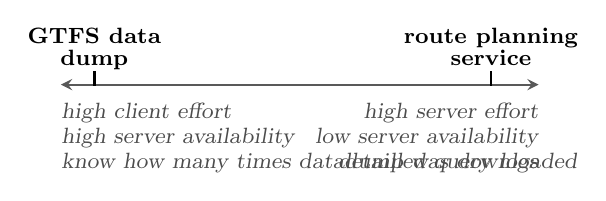
\begin{tikzpicture}[
    x=.005\textwidth,
    y=.1cm,
    axis/.style={
      line width=.8pt,
      stealth-stealth,
      color=black!65,
    },
    axislabel/.style={
      inner sep=0,
      font=\slshape\fontsize{8}{9}\selectfont,
      color=black!70,
    },
    tick/.style={
      line width=1pt,
    },
    ticklabel/.style={
      anchor=south,
      inner sep=0,
      align=center,
      font=\bfseries\fontsize{8}{8}\selectfont,
      text depth=0pt,
    },
  ]
    \newcommand\tick[2]{%
      \draw[tick] (#1, 1.7) -- (#1, -.4pt);
      \node[ticklabel] at (#1, 2.4) {#2};
    }
    \newcommand\vaguetick[1]{%
      \draw[tick,densely dotted] (#1, 1.7) -- (#1, -.4pt);
    }

    \draw[axis] (-100, 0) -- (0, 0);
    \node[axislabel,align=left,anchor=north west] at (-100, -2.3)
    {
%      generic requests\\
      high client effort\\
      high server availability\\
      know how many times datadump was downloaded
    };
    \node[axislabel,align=right,anchor=north east] at (0, -2.3)
    {
%      specific requests\\
      high server effort\\
      low server availability\\
      detailled query logs
    };

    \tick{-93}{GTFS data\\dump}
    \tick{-10}{route planning\\service}
%    \tick{-32}{Linked\\Connections}

   % \vaguetick{-84}
   % \vaguetick{-52}
   % \vaguetick{  5}
   % \vaguetick{-10}
   % \vaguetick{ 28}
   % \vaguetick{ 55}

   %\node[align=center,font=\fontsize{8}{9}\selectfont\bfseries] at (0, -8.3)
   %   {various types of\\Linked Data Fragments};
  \end{tikzpicture}
  \caption{
    This axis illustrates two extremes. With GTFS data dumps, the data reusers do all the work, and no query logs can be gathered. With route planning services, the servers need to do all the work, yet detailled query logs can be studied.
  }
  \label{fig:LDFAxis1}
\end{figure}

Getting indications of people flows through public transit networks is a challenge.
The data is tedious to get, mainly with public transit systems where passengers don't have to check-in and check-out.
Nevertheless, people are calculating their intended routes by using the Web.
The \emph{iRail} project\footnote{\url{http://hello.irail.be}} started in 2008 to make the data of the Belgian railway accessible for developers.
Ever since, the project offers developer both a GTFS data dump for third party apps and a route planning API.

In this paper, we give a small overview of related work trying to gather data for flow analysis.
Next, we study the iRail query logs to find out whether we can find interesting patterns.
Finally, we look at Linked Connections~\cite{lc}, a proposed new way of publishing queryable public transit data, and whether we would still be able to have an indication of the transit flows with a Linked Data Fragments~\cite{ldf} approach.

\section{Related work}
\label{sec:relwork}

\emph{Flow analysis} is a topic of theoretical interest and practical importance in various disciplines. 
Flow analysis is conventionally conducted to study spatial dynamics and identify routine patterns in the movement of people.
For instance, interest in modelling traffic flows emerged from the strain placed on urban transportation systems during peak hours~\cite{roth,ferreira}.
Likewise, insight into routine travel patterns is crucial for the conceptualisation of functional urban areas~\cite{servillo,sykora}, urban hierarchies~\cite{christaller} and other territorial structures.

Over the past decade, large datasets have become increasingly commonplace due to the proliferation of sensor networks and portable devices like smartphones.
Termed ``Big Data'' due to the large volume of data records that emerge from real-time sensing\cite{kitchin}, such datasets typically contain information of activities or processes linked to the space and time where they occur.
In the domain of ``Smart City'' research, much has been accomplished with the use of ``Big Data'' to monitor human movement.
Smart card data from public transport systems~\cite{roth,beecham}, taxi journeys~\cite{ferreira} as well as cellular call data~\cite{sevtsuk} have provided planners with new opportunities to develop greater understanding of mobility patterns in urban environments~\cite{batty}.

\section{Gathering the logs}
\label{sec:logs}

In 2013, we have started to use a MySQL table to store each request in a table, including User-Agent string, the timestamp, whether or not the request succeeded, the departure station and the desired station of arrival.
From an export of this table, we have filtered out only the route plannning queries that succeeded.
The resulting dataset, used for the rest of this paper, can be downloaded at \todo{\url{http://datawijs.be/iraillogs.zip}}.

We have cleaned this data by removing the requests done by harvesters or search engine bots.
Thanks to the user agents, this was a fairly straight-forward operation.
The remainder of the file delivers an average of 3000 route planning queries a day, which we can use an an indication of travel intensities.

Today, iRail publishes the most recent 1000 requests done on the API as open data, each second, at \url{http://api.irail.be/logs/}.
This amounts today to an average of 200k queries to the API per day, as the API gained popularity thanks to apps like \emph{BeTrains}\footnote{\todo{\url{http://...}}} and \emph{Railer}\footnote{\todo{\url{http://...}}}.

\section{Looking for patterns}
\label{sec:method}

There are obvious caveats associated with the use of such data as proxy for actual statistical counts.

\section{Results}
\label{sec:results}
\todo{
We can also observe the effect of "density" in Flanders where people move from the rural towards cities. Look at weekday-mornings: commuting towards Gent, Brussels, Antwerp. This is not as obvious in the Walloon region (except for Liege). The reverse occurs on weekday-evenings. Local patterns can also be observed and this corresponds to what we know: "cities are the central hubs".
Walloon region: everything converges on Brussels
I found that whereas there's almost no movement from Antwerp city in the week to West Flanders, there is movement from Antwerp in the weekend to the coast and back. 
}

\todo{This pair of chord diagrams capture the aggregated number of queries made between any two stations on weekdays and weekends between 6 to 9 in the morning. The chords that link two distinct stations, are coloured coded by region and proportionately scaled to the number of queries from a station of origin to a destination. For instance, approximately 3,530 queries were made from Leuven to Brussels than in the opposite direction (approximately 1,530) on weekdays. Reading both diagrams in this manner reveals the complexity of movement on the rail system and the significance of cities in daily travel. Brussels serves as the principal centre of rail activity in general, yet its centrality is more distinctive for the walloon region than Flanders. Queries from Walloonia with exception to Liege, are generally made from provincial stations towards Brussels instead of their respective provincial capitals. Queries in Flanders, on the hand, tend to be distributed among major cities otherwise known as the Flemish Diamond (Vlaamse Ruit), a network of four metropolitan areas in Belgium comprised of Ghent, Brussels, Antwerp and Leuven. The difference between both patterns appear to correspond with existing measures of population density, providing valuable insight and alternative perspectives into the function of cities in rural and urban settings.}

\todo{add a couple of nice images with explanation here}

\subsection{Pattern 1: ...}
\label{sec:pattern1}

\subsection{Pattern 2: ...}
\label{sec:pattern2}

\section{Publishing transport data and the impact on query logs}
\label{sec:publishing}

Publishing public transport data today happens in two ways: by publishing a data dump of the timetables or by hosting a public route planning service.
Linked Data Fragments~\cite{ldf} is a way to think about data publishing as a set of trade-offs between client and servers.
These trade-offs can be mapped on an axis, cfr. \cref{fig:LDFAxis2}, in which the 2 extremes are identified as: the server does all the processing versus the client does all the processing.

Also for query logs we can make the same trade-off, in which the 2 extremes are the server knows only when someone downloads the entire datadump versus the server has a detailled query log.
In this paper, we have studied the query logs of an API s

%label: fig:LDFAxis2

% Linked Data Fragments axis
\begin{figure}[t]
  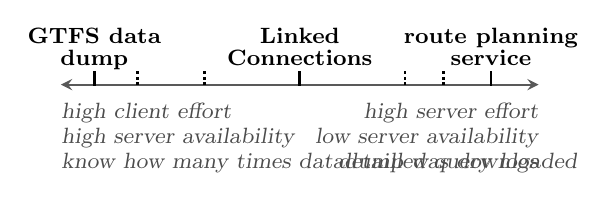
\begin{tikzpicture}[
    x=.005\textwidth,
    y=.1cm,
    axis/.style={
      line width=.8pt,
      stealth-stealth,
      color=black!65,
    },
    axislabel/.style={
      inner sep=0,
      font=\slshape\fontsize{8}{9}\selectfont,
      color=black!70,
    },
    tick/.style={
      line width=1pt,
    },
    ticklabel/.style={
      anchor=south,
      inner sep=0,
      align=center,
      font=\bfseries\fontsize{8}{8}\selectfont,
      text depth=0pt,
    },
  ]
    \newcommand\tick[2]{%
      \draw[tick] (#1, 1.7) -- (#1, -.4pt);
      \node[ticklabel] at (#1, 2.4) {#2};
    }
    \newcommand\vaguetick[1]{%
      \draw[tick,densely dotted] (#1, 1.7) -- (#1, -.4pt);
    }

    \draw[axis] (-100, 0) -- (0, 0);
    \node[axislabel,align=left,anchor=north west] at (-100, -2.3)
    {
%      generic requests\\
      high client effort\\
      high server availability\\
      know how many times datadump was downloaded
    };
    \node[axislabel,align=right,anchor=north east] at (0, -2.3)
    {
%      specific requests\\
      high server effort\\
      low server availability\\
      detailled query logs
    };

    \tick{-93}{GTFS data\\dump}
    \tick{-10}{route planning\\service}
    \tick{-50}{Linked\\Connections}

    \vaguetick{-84}    \vaguetick{-70}
    \vaguetick{-10}
    \vaguetick{-28}
    \vaguetick{-20}

   %\node[align=center,font=\fontsize{8}{9}\selectfont\bfseries] at (0, -8.3)
   %   {various types of\\Linked Data Fragments};
  \end{tikzpicture}
  \caption{This axis extends \cref{fig:LDFAxis1} with Linked Connections: a different choice of trade-offs for route planning advice over the Web.
  }
  \label{fig:LDFAxis2}
\end{figure}

\todo{Also in USEWOD2014 there was a paper on LDF and how we could know which SPARQL queries needed to be solved}

Thoughts on publishing transport data on the web and query logs in the case of GTFS, Linked Connections\cite{lc} (linked data fragments\cite{ldf}) and webservices.

\section{Conclusion and discussion}
\label{sec:conclusion}

Query logs are very interesting

% Fix spacing after References header (as line 1308 of sig-alternate.cls breaks it)
\let\oldsection\section
\renewcommand{\section}[2][1]{\oldsection{#1}\vspace{-3pt}}

\bibliographystyle{abbrv}
\bibliography{refs}
\end{document}
